\begin{frame}
\frametitle{Базовая модель: Dreamer}
\begin{columns}
\begin{column}{0.7\textwidth}
% \begin{framefont}{}
\begin{itemize}
    \item Dreamer\footnotemark[1] представляет собой вариационный автоэнкодер (VAE), кодирующий наблюдения и награды  
    \item Он состоит из
    \begin{itemize}
        \item модели репрезентации (энкодера) $q(s_t\mid s_{t-1}, a_{t-1}, o_{t})$
        \item модель среды $p(s_t \mid s_{t-1}, a_{t-1})$
        \item модель наблюдений (декодер изображений) $p(o_t\mid s_t)$
        \item модели награды (декодер наград) $p(r_t\mid s_t)$
    \end{itemize}
    \item Наблюдения $o_{1:T}$ считаются не марковскими, в связи с чем  VAE выводит марковские состояния $s_t$
    \item Стратегия и критик тренируются на траекториях, полученных в "воображении" модели, полученных при помощи модели среды $p(s_t\mid s_{t-1}, a_{t-1})$
\end{itemize}
% \end{framefont}
\end{column}
\begin{column}{0.4\textwidth}

\begin{figure}
\centering
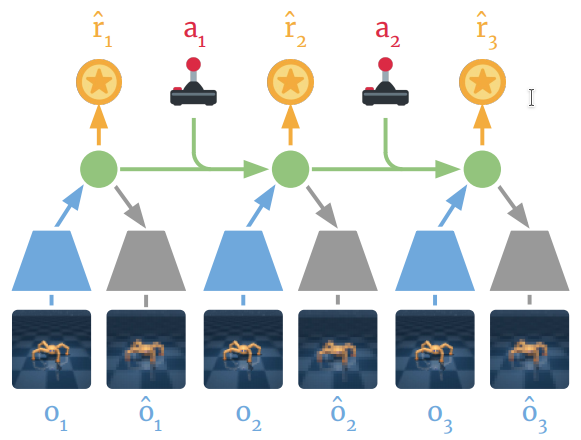
\includegraphics[width=\linewidth]{images/dreamer/1.png}\\
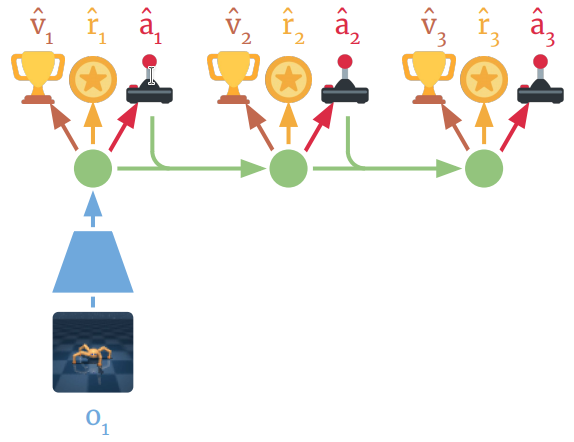
\includegraphics[width=\linewidth]{images/dreamer/2.png}
% \caption{Графическая модель RSSM}
% \label{figM:2}
\end{figure}
\end{column}
\end{columns}
\footnotetext[1]{Danijar Hafner et al. “Dream to Control: Learning Behaviors by Latent Imagination”. In:
ICLR 2020}
\end{frame}